\documentclass[10pt, fleqn]{article}
\usepackage[a4paper,margin=0.5in]{geometry}
\usepackage{multicol}
\usepackage{amsmath, amssymb}
\usepackage{titlesec}
\usepackage{float}
\usepackage{amsfonts, bm, graphicx}
\usepackage{enumitem}
\usepackage[font=small, skip=4pt]{caption}

\setlength{\abovedisplayskip}{6pt}
\setlength{\belowdisplayskip}{6pt}
\setlength{\abovedisplayshortskip}{4pt}
\setlength{\belowdisplayshortskip}{4pt}

\setlength{\textfloatsep}{8pt plus 2pt minus 2pt}
\setlength{\intextsep}{6pt plus 2pt minus 2pt}
\setlength{\floatsep}{8pt plus 2pt minus 2pt}

\setlength{\mathindent}{0pt}

\titleformat{\section}{\large\bfseries}{}{0em}{}
\titleformat{\subsection}{\normalsize\bfseries}{}{0em}{}
% Uppercase Volume with thicker, higher line
\newcommand{\vol}{\mathord{\text{\ooalign{\hidewidth $V$\hidewidth\cr\kern-0.5pt\raisebox{0.8ex}{\rule[0pt]{1em}{0.5pt}}}}}}

% Lowercase Volume with built-in shifts
\newcommand{\svol}{%
  \mathord{\text{\ooalign{%
    \hspace{0.1em}$v$\cr         % built-in horizontal shift of 'v'
    \hspace{-0.02em}\rule[0.6ex]{0.8em}{0.5pt} % built-in horizontal shift of the bar, vertical raise, length, thickness
  }}}%
}
\begin{document}

\begin{center}
    \Large \textbf{Thermodynamics Formula Sheet} \\
    \normalsize Exam 1
\end{center}
    \section*{Units and Conversions}
    \vspace{-1em}
\begin{multicols}{2}\noindent
\textbf{SI Prefixes}
\makeatletter
\@fleqnfalse
\makeatother
\[
\begin{array}{ll@{\qquad}ll}
\text{femto (f)} &= 10^{-15} & \text{deca (da)} &= 10^{1} \\
\text{pico (p)} &= 10^{-12} & \text{hecto (h)} &= 10^{2} \\
\text{nano (n)} &= 10^{-9}  & \text{kilo (k)} &= 10^{3} \\
\text{micro ($\mu$)} &= 10^{-6} & \text{mega (M)} &= 10^{6} \\
\text{milli (m)} &= 10^{-3} & \text{giga (G)} &= 10^{9} \\
\text{centi (c)} &= 10^{-2} & \text{tera (T)} &= 10^{12} \\
\text{deci (d)} &= 10^{-1}  & \text{peta (P)} &= 10^{15}
\end{array}
\]
\makeatletter
\@fleqntrue
\makeatother
\textbf{Atmospheric Pressure}
\[\begin{aligned}
1 \text{ atm} &= 101.325 \text{ kPa} \\
&= 1.01325 \text{ bar} \\
&= 760 \text{ Torr} \\
&= 760 \text{ mmHg} \\
&= 29.92 \text{ inHg} \\
&= 14.696 \text{ psi}\\
&= 10.33 \text{ m H}_2\text{O (at 4$^\circ$C)} \\
\end{aligned}\]
\textbf{Pressure Conversions}
\[1\,\text{Pa} = 1\,\text{N/m}^2\]
\[1\, \text{ bar} = 10^{5}\, \text{ Pa}\]
\[1\, \text{ psi} = 6.89476 \times 10^{3}\, \text{ Pa}\]
\[1\, \text{ Torr} = 133.322\, \text{ Pa}\]
\[1\, \text{ mmHg} = 133.322\, \text{ Pa}\]
\[1\, \text{ inHg} = 3.38639 \times 10^{3}\, \text{ Pa}\]
\textbf{Gauge vs Absolute Pressure}
\[P_{\text{gauge}} = P_{\text{absolute}} - P_{\text{atmospheric}}\]
\[P_{\text{vacuum}} = P_{\text{atmospheric}} - P_{\text{absolute}}\]
\underline{Note:} Generally, gauge pressures already account for atmospheric pressure, and thus reads zero when open to the atmosphere.\\
\textbf{Temperature Conversions}
\begin{itemize}[label=\textbullet]
    \item Absolute temperature conversions
    \begin{itemize}[label=\textopenbullet]
        \item $T_{K} = T_{^\circ C} + 273.15$
        \item $T_{^\circ R} = T_{^\circ F} + 459.67$
        \item $T_{^\circ F} = \frac{9}{5}T_{^\circ C} + 32$
        \item $T_{^\circ R} = \frac{9}{5}T_{K}$
    \end{itemize}
    \item Temperature difference conversions
    \begin{itemize}[label=\textopenbullet]
        \item $\Delta K = \Delta ^\circ C$
        \item $\Delta ^\circ R = \Delta ^\circ F$
        \item $\Delta ^\circ F = \frac{9}{5}\Delta ^\circ C$
        \item $\Delta ^\circ R = \frac{9}{5}\Delta K$
    \end{itemize}
\end{itemize}
\section*{Density and Specific Gravity}
\[\rho = \frac{m}{\vol}\quad \text{(density)}\]
\[\svol = \frac{\vol}{m} = \frac{1}{\rho} \quad \text{(specific volume)}\]
\textbf{Specific gravity} is defined as a relative density compared to water (at 4$^\circ$C) where $\rho_{water} = 1000\,\text{kg/m}^3$:
\[\boxed{SG = \frac{\rho_{fluid}}{\rho_{water}} \implies \rho_{fluid} = SG \cdot \rho_{water}}\]
\textbf{Specific Weight}
\[\gamma_s = \rho g \quad \text{(specific weight)}\]
Where hydrostatic pressure can be written as $P = \gamma_s h$\\\\
\textbf{Slugs and lbm}
\[\left[\frac{1\,\text{lbf}}{32.174\,\frac{\text{lbm}\cdot\text{ft}}{\text{s}^2}}\right],\quad
\left[\frac{1\,\text{slug}}{32.174\,\text{lb,}}\right], \quad
\left[\frac{1\,\text{lbf}}{1\,\frac{\text{slug}\cdot\text{ft}}{\text{s}^2}}\right]\]
\textbf{Energy Units}\\
1 Btu = 778.169 ft$\cdot$lbf = 1055.06 J\\\\
\textbf{Work Units}\\
1 hp = 550 ft$\cdot$lbf/s = 745.7 W\\\\
\textbf{Distance}\\
1 mile = 5280 ft\\\\
\textbf{Ideal Gas Law}
\[ P \, \svol = R \, T, \quad
R = \frac{\bar{R}}{M} \quad \text{(specific gas constant, J/kg·K)}\]
\[P\vol = mRT \quad \text{(using total volume and mass)}\]
\textbf{Universal gas constant:}  $\bar{R} = 8.314$ J/(mol·K)
\begin{center}
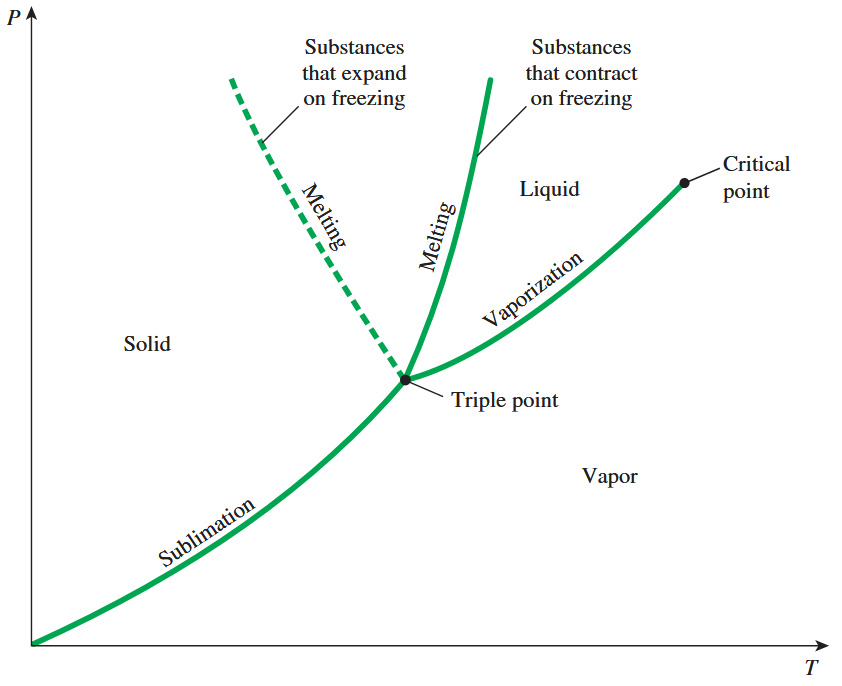
\includegraphics[width=0.5\textwidth]{../../PT.png}
\end{center}
\end{multicols}\newpage
\begin{multicols}{2}
\begin{center}
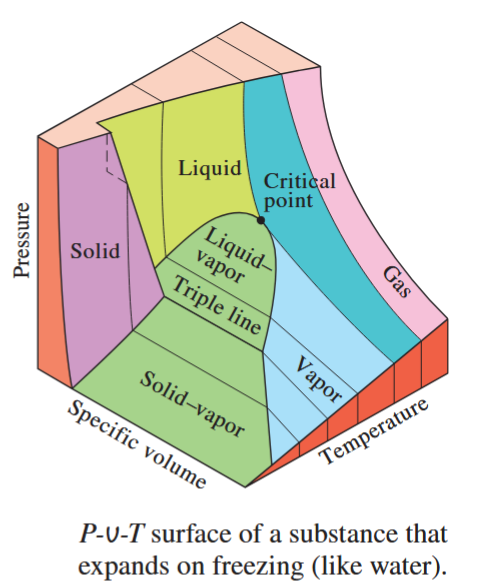
\includegraphics[width=0.35\textwidth]{PVT - Copy.png}
\end{center}
\begin{center}
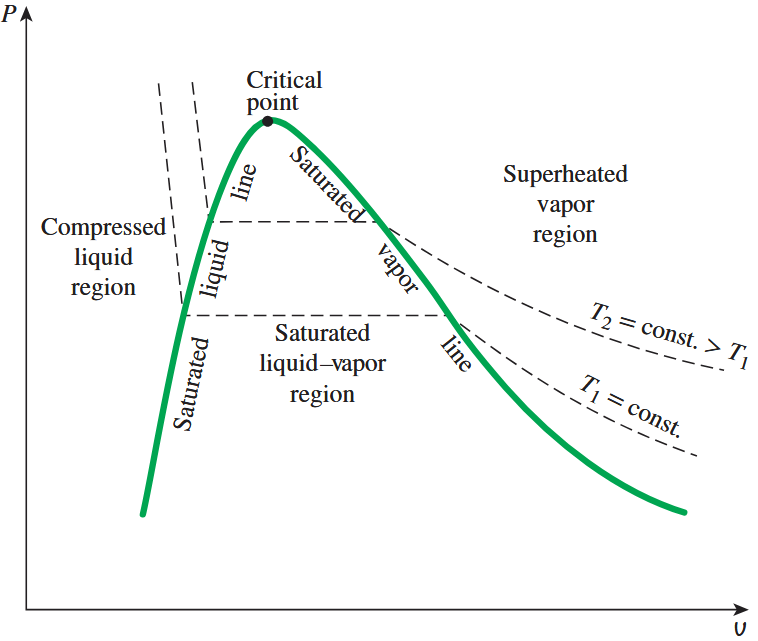
\includegraphics[width=0.35\textwidth]{../../PV.png}
\end{center}
\begin{center}
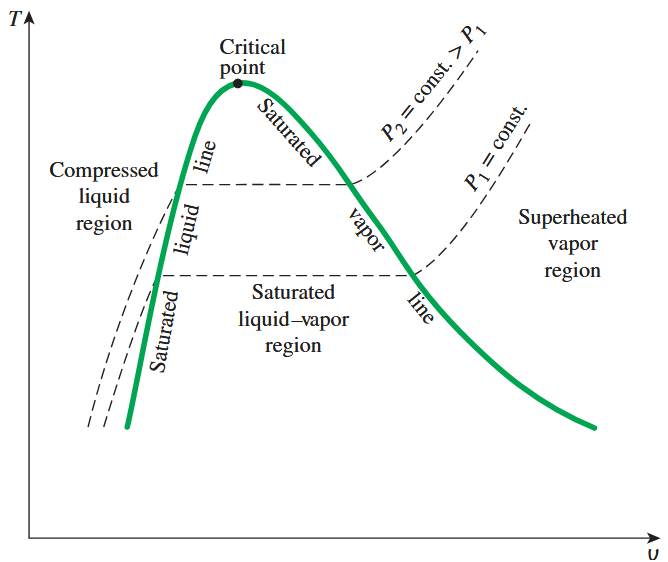
\includegraphics[width=0.35\textwidth]{../../TV.png}
\end{center}
\begin{center}
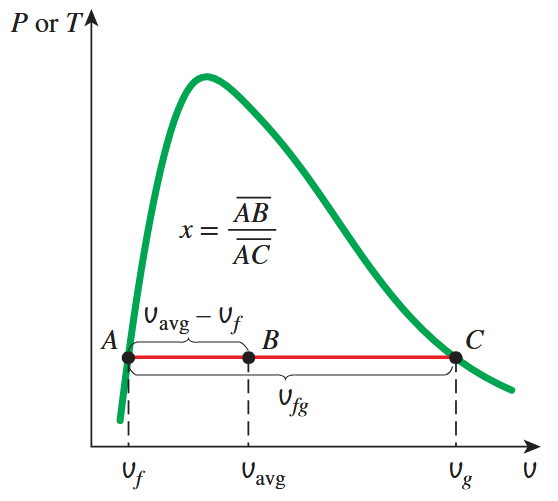
\includegraphics[width=0.35\textwidth]{../../Quality.png}
\end{center}
\textbf{Pressure Relations}
\[P = \frac{F}{A} = \rho g h \quad \text{(hydrostatic pressure)}\]
\[P_1 = P_2 \quad \Rightarrow \quad \frac{F_1}{A_1} = \frac{F_2}{A_2} \quad \text{(Pascal's Law)}\]
\[\Delta P = \rho g h \quad \text{(multi-fluid manometer)}\]
(add downward, subtract upward)\\
\textbf{Energy Definitions}
\[e = u + \frac{1}{2}v^2 + gh \quad \text{(specific total energy = internal + KE + PE)}\]
\[e_\text{mech} = \frac{P}{\rho} + \frac{1}{2}v^2 + gh \quad \text{(specific mechanical energy)}\]
\textbf{First Law (Closed System)}
\[\Delta U = Q - W \quad \text{(energy balance for closed system)}\]
\[\dot E_{in} - \dot E_{out} = \frac{dE_{system}}{dt} \quad \text{(rate form)}\]
\textbf{First Law (Open System)}
\[\frac{dE}{dt} = \dot{Q}-\dot{W}+
\underbrace{\sum \dot{m_i}\left[h_i+\frac{1}{2}V_i^2+g z_i\right]}_{\text{Inlet}}
-\underbrace{\sum \dot{m_e}\left[h_e+\frac{1}{2}V_e^2+g z_e\right]}_{\text{Outlet}}\]
For steady state process with no heat transfer:
\[\dot{W}=\dot{m}e_\text{mech}\quad \]
\[\dot W = \dot m \frac{\Delta P}{\rho} = \dot \vol \Delta P \quad \text{(pump power w/ no change in KE or PE)}\]
\textbf{Mass \& Flow Relations}
\[\dot m = \rho \dot \vol = \rho A v_{avg} \quad \text{(mass flow rate)}\]
\[\dot E = \dot m e \quad \text{(energy flow rate)}\]
\textbf{Enthalpy}
\[h = u + P\svol,\quad \svol = \frac{1}{\rho} \quad \text{(specific enthalpy)}\]
\textbf{Work}
\[W = \int F \cdot dx, \quad \dot{W}=F\cdot v\quad\text{(general)}\]
\[W = VI\Delta t, \quad \dot W = VI = RI^2 = \frac{V^2}{R}\quad\text{(electrical)}\]
\[W = 2\pi n T, \quad \dot W = 2\pi \dot n T \quad \text{(shaft)}\]
\[W = \frac{1}{2}k(x_2^2 - x_1^2) \quad \text{(spring work)}\]
\textbf{Heat Transfer}
\[Q = \int \dot Q\,dt = \dot Q \Delta t \quad \text{(total heat transferred)}\]
\[\dot Q = kA \frac{\Delta T}{\Delta x} \quad \text{(conduction)}\]
\[\dot Q = hA(T_s - T_f) \quad \text{(convection)}\]
\textbf{Phase Change \& Saturation}
\[h_{fg} = h_g - h_f \quad \text{(latent heat of vaporization)}\]
\[x = \frac{m_g}{m_f + m_g} \quad \text{(quality definition)}\]
\[y_\text{avg} = y_f + x(y_g - y_f) \quad \text{(relation for }\svol, h, u)\]
\[x = \frac{y_\text{avg} - y_f}{y_g - y_f} \quad \text{(solve for quality)}\]
\textbf{Compressed Liquid Approximation}
\[y(T,P) \approx y_f(T) \quad \text{(use saturated liquid at same T)}\]
\end{multicols}









\end{document}
